%Version 3 December 2023
% See section 11 of the User Manual for version history
%
%%%%%%%%%%%%%%%%%%%%%%%%%%%%%%%%%%%%%%%%%%%%%%%%%%%%%%%%%%%%%%%%%%%%%%
%%                                                                 %%
%% Please do not use \input{...} to include other tex files.       %%
%% Submit your LaTeX manuscript as one .tex document.              %%
%%                                                                 %%
%% All additional figures and files should be attached             %%
%% separately and not embedded in the \TeX\ document itself.       %%
%%                                                                 %%
%%%%%%%%%%%%%%%%%%%%%%%%%%%%%%%%%%%%%%%%%%%%%%%%%%%%%%%%%%%%%%%%%%%%%

%%\documentclass[referee,sn-basic]{sn-jnl}% referee option is meant for double line spacing

%%=======================================================%%
%% to print line numbers in the margin use lineno option %%
%%=======================================================%%

%%\documentclass[lineno,sn-basic]{sn-jnl}% Basic Springer Nature Reference Style/Chemistry Reference Style

%%======================================================%%
%% to compile with pdflatex/xelatex use pdflatex option %%
%%======================================================%%

%%\documentclass[pdflatex,sn-basic]{sn-jnl}% Basic Springer Nature Reference Style/Chemistry Reference Style


%%Note: the following reference styles support Namedate and Numbered referencing. By default the style follows the most common style. To switch between the options you can add or remove “Numbered” in the optional parenthesis. 
%%The option is available for: sn-basic.bst, sn-vancouver.bst, sn-chicago.bst%  
 
%%\documentclass[pdflatex,sn-nature]{sn-jnl}% Style for submissions to Nature Portfolio journals
%%\documentclass[pdflatex,sn-basic]{sn-jnl}% Basic Springer Nature Reference Style/Chemistry Reference Style
\documentclass[pdflatex,sn-mathphys-num]{sn-jnl}% Math and Physical Sciences Numbered Reference Style 
%%\documentclass[pdflatex,sn-mathphys-ay]{sn-jnl}% Math and Physical Sciences Author Year Reference Style
%%\documentclass[pdflatex,sn-aps]{sn-jnl}% American Physical Society (APS) Reference Style
%%\documentclass[pdflatex,sn-vancouver,Numbered]{sn-jnl}% Vancouver Reference Style
%%\documentclass[pdflatex,sn-apa]{sn-jnl}% APA Reference Style 
%%\documentclass[pdflatex,sn-chicago]{sn-jnl}% Chicago-based Humanities Reference Style

%%%% Standard Packages
%%<additional latex packages if required can be included here>

\usepackage{graphicx}%
\usepackage{multirow}%
\usepackage{amsmath,amssymb,amsfonts}%
\usepackage{amsthm}%
\usepackage{mathrsfs}%
\usepackage[title]{appendix}%
\usepackage{xcolor}%
\usepackage{textcomp}%
\usepackage{manyfoot}%
\usepackage{booktabs}%
\usepackage{algorithm}%
\usepackage{algorithmicx}%
\usepackage{algpseudocode}%
\usepackage{listings}%
\usepackage{enumitem}%
\usepackage{afterpage}%


%%%%

%%%%%=============================================================================%%%%
%%%%  Remarks: This template is provided to aid authors with the preparation
%%%%  of original research articles intended for submission to journals published 
%%%%  by Springer Nature. The guidance has been prepared in partnership with 
%%%%  production teams to conform to Springer Nature technical requirements. 
%%%%  Editorial and presentation requirements differ among journal portfolios and 
%%%%  research disciplines. You may find sections in this template are irrelevant 
%%%%  to your work and are empowered to omit any such section if allowed by the 
%%%%  journal you intend to submit to. The submission guidelines and policies 
%%%%  of the journal take precedence. A detailed User Manual is available in the 
%%%%  template package for technical guidance.
%%%%%=============================================================================%%%%

%% as per the requirement new theorem styles can be included as shown below
%\theoremstyle{thmstyleone}%
\newtheorem{theorem}{Theorem}%  meant for continuous numbers
%%\newtheorem{theorem}{Theorem}[section]% meant for sectionwise numbers
%% optional argument [theorem] produces theorem numbering sequence instead of independent numbers for Proposition
\newtheorem{proposition}[theorem]{Proposition}% 
%%\newtheorem{proposition}{Proposition}% to get separate numbers for theorem and proposition etc.

%\theoremstyle{thmstyletwo}%
\newtheorem{example}{Example}%
\newtheorem{remark}{Remark}%

%\theoremstyle{thmstylethree}%
\newtheorem{definition}{Definition}%

\raggedbottom
%%\unnumbered% uncomment this for unnumbered level heads

\begin{document}

\title[Article Title]{Leveraging Graph-Based Learning for Credit Card Fraud Detection:  A comparative study of classical, deep learning and graph-based approaches.}

%%=============================================================%%
%% GivenName	-> \fnm{Joergen W.}
%% Particle	-> \spfx{van der} -> surname prefix
%% FamilyName	-> \sur{Ploeg}
%% Suffix	-> \sfx{IV}
%% \author*[1,2]{\fnm{Joergen W.} \spfx{van der} \sur{Ploeg} 
%%  \sfx{IV}}\email{iauthor@gmail.com}
%%=============================================================%%
\author*[1]{\fnm{Sunisha} \sur{Harish}} \email{sunishaharish@gwu.edu}
\equalcont{These authors contributed equally to this work.}

\author[1]{\fnm{Chirag} \sur{Lakhanpal}} \email{chiraglakhanpal@gwu.edu}
\equalcont{These authors contributed equally to this work.}

\author[1]{\fnm{Amir} \sur{Hossein Jafari}} \email{ajafari@gwu.edu}

\affil[1]{\orgdiv{Department of Data Science}, \orgname{The George Washington University}, \state{Washington DC 20052}, \country{USA}}

%%==================================%%
%% Sample for unstructured abstract %%
%%==================================%%

\abstract{Credit card fraud results in staggering financial losses amounting to billions of dollars annually, impacting both merchants and consumers. In the light of the escalating prevalence of digital crime and online fraud, it is important for organizations to implement robust and advanced technology to efficiently detect fraud and mitigate the issue. Contemporary solutions heavily rely on machine learning (ML) and deep learning (DL) methods to handle such tasks. While these methods have been effective in many aspects of fraud detection, they may not always be sufficient for credit card fraud detection as they aren’t adaptable to detect complex relationships when it comes to transaction. Fraudsters, for example, might set up many coordinated accounts to avoid triggering limitations on individual accounts. In the context of fraud detection, the ability of Graph Neural Networks (GNN’s) to aggregate information contained within the local neighbourhood of a transaction enables them to identify larger patterns that may be missed by just looking at a single transaction. In this research, we conduct a thorough analysis to evaluate the effectiveness of GNNs in improving fraud detection over traditional Machine Learning and Deep Learning methods. We first build an heterogenous graph architecture with the source, transaction, and destination as our nodes. Next, we leverage Relational Graph Convolutional Network to learn the representations of nodes in our graph and perform node classification on the transaction node. Our experimental results demonstrate that GNN outperforms traditional and deep learning methods.
}

%%================================%%
%% Sample for structured abstract %%
%%================================%%

% \abstract{\textbf{Purpose:} The abstract serves both as a general introduction to the topic and as a brief, non-technical summary of the main results and their implications. The abstract must not include subheadings (unless expressly permitted in the journal's Instructions to Authors), equations or citations. As a guide the abstract should not exceed 200 words. Most journals do not set a hard limit however authors are advised to check the author instructions for the journal they are submitting to.
% 
% \textbf{Methods:} The abstract serves both as a general introduction to the topic and as a brief, non-technical summary of the main results and their implications. The abstract must not include subheadings (unless expressly permitted in the journal's Instructions to Authors), equations or citations. As a guide the abstract should not exceed 200 words. Most journals do not set a hard limit however authors are advised to check the author instructions for the journal they are submitting to.
% 
% \textbf{Results:} The abstract serves both as a general introduction to the topic and as a brief, non-technical summary of the main results and their implications. The abstract must not include subheadings (unless expressly permitted in the journal's Instructions to Authors), equations or citations. As a guide the abstract should not exceed 200 words. Most journals do not set a hard limit however authors are advised to check the author instructions for the journal they are submitting to.
% 
% \textbf{Conclusion:} The abstract serves both as a general introduction to the topic and as a brief, non-technical summary of the main results and their implications. The abstract must not include subheadings (unless expressly permitted in the journal's Instructions to Authors), equations or citations. As a guide the abstract should not exceed 200 words. Most journals do not set a hard limit however authors are advised to check the author instructions for the journal they are submitting to.}

\keywords{Credit card fraud, Graph neural networks, Node classification, RGCN, Deep learning, Machine learning}

%%\pacs[JEL Classification]{D8, H51}

%%\pacs[MSC Classification]{35A01, 65L10, 65L12, 65L20, 65L70}

\maketitle

\section{Introduction}\label{sec1}

With the growing upsurge in credit card payments, credit card fraud has become the most common form of identity theft. Credit card fraud occurs when someone uses another person’s credit card or credit card information to buy something or access an account without permission.  According to Federal Trade Commission Data \cite{ftc2024} a loss of more than \$10 billion to fraud was reported by the consumers in 2023. This data signifies a 14\% increase over losses documented in 2022. There are different types of credit card frauds that can occur \cite{capitalone2024}. One is the fraud committed over phone or online where the fraudster has the card details but not the card. Another way is credit card skimming, where a fake or cloned card id can be created using someone else’s information. Fraudsters can also get hold of a customer’s personal information and use them to access their credit card account or apply for a new card in their name. Fraud can also occur through a lost or stolen credit card. Although the ratio of fraud transactions is very low, credit card fraud undermines consumer trust, leading to reduced spending and increased costs for businesses, ultimately hindering economic growth and stability. It also imposes financial burdens on individuals and businesses, disrupts operations, and introduces legal and regulatory complexities.

In this paper, we present our solution to tackle the problem of credit card fraud using machine learning, deep learning, and graph neural networks. We are using the Tabformer dataset provided by IBM \cite{ibm2021} to demonstrate this workflow. The TabFormer dataset is a synthetic credit card transaction dataset, consisting of around 24 million unique transactions and around 0.1\% of fraudulent samples. The rest of the paper is organized as follows: Section 2 covers the background and related work done on fraud detection. Section 3 describes the methodology used. Section 4 covers the experimentation and results. The last section concludes our work with the scope for future work.

\section{Background and Related Work}\label{sec2}

\subsection{Classical and Deep Learning Approaches}\label{subsec2}

Fraud detection has been a great motivation for researchers to find a solution. Numerous methods have been proposed and tested to detect and prevent fraud. Their primary function is to utilize historical data to automatically detect fraudulent transactions. While they excel at identifying established fraud patterns, they struggle dealing with unfamiliar types of fraud. Our literature review focused on researching the work performed on credit card fraud detection using traditional, deep learning and graph neural networks.

Methods using machine learning models have been compared, these models have achieved much success \cite{awoyemi2017}. Classical algorithms such as, Decision Tree (DT), Random Forest (RF) and Gradient Boosting Classifier (GBC) have proven useful \cite{mohbey2022}. Random Forest and AdaBoost Algorithm were compared \cite{sailusha2020} after applying SMOTE to balance the dataset and the RF algorithm achieved better precision, recall and F1-score. Paper \cite{varmedja2019} benchmarked several machine learning models along with MLP Classifier on a real-world credit card fraud dataset and found that the Random Forest classifier performed best after applying oversampling and feature selection techniques to the highly imbalanced data. These studies proved that classical models perform very well when data imbalance is handled using proper techniques. Classical models tend to bias towards the majority class and overfit the minority class and hence perform poorly on unbalanced data. 

Ensemble techniques such as XGBoost demonstrate a superior ability to effectively handle imbalanced data distributions compared to traditional machine learning models, as evidenced by their considerably better performance metrics reported in the paper \cite{mohbey2022}. XGBoost uses gradient boosting which builds ensemble models in a sequential manner and handles weighted instances, allowing it to better adapt to the imbalanced class distributions. Ensemble learning methods using LightGBM and LightMort along with simple and weighted average methods by using the feature importance and feature engineering property of the LightGBM algorithm to improve efficiency \cite{bakhtiari2023}. KNN, LDA and LR have been combined to effectively enhance recall in credit card fraud detection \cite{chung2023}.


Classical models may produce great results, but they require handling the data imbalance, and it is difficult to model the relationships between different entities to capture complex fraud patterns. They focus on direct relationships potentially overlooking fraudulent patterns embedded with broader complexities.

In recent years, deep learning approaches have also been extensively explored for credit card fraud detection, in addition to traditional machine learning models. Deep learning is an actively researched area that shows potential in enhancing fraud detection performance, especially with larger future datasets.
Various classical and deep learning methods have been compared to understand which method yields better performance for fraud detection \cite{alarfaj2022credit}.

Paper \cite{hassan2020} compared machine learning algorithms along with Bi-LSTM and Bi-GRU and much better results were achieved with the deep learning methods. Methods such as CNN and LSTM have been widely used for image classification and Natural Language Processing respectively due to their ability to handle massive datasets. CNN and LSTM have also proved to be quite efficient in delivering promising results for fraud detection as CNN captures spatial patterns well and LSTM as a sequence learner is useful in capturing time in transactions\cite{nguyen2020}. LSTM as a sequence learner has been compared with Random Forest (a static learner) on online and offline transactions and their behaviour has been studied \cite{jurgovsky2018}.

Hybrid approaches combining deep learning with other techniques have been explored to counter class imbalance. CCFD-Net used a hybrid architecture of 1D Covolutional Network and the residual neural network (Res-Net) \cite{liu2021}. The study showed that hybrid architecture produces much better results and can be used for numerical data classification. Traditional and deep learning models have also been used to create ensemble methods where the results of individual classifiers have been combined to get the final classifier results \cite{sahithi2022} \cite{sohony2018}.

Paper \cite{hilal2022} explored various classical models, deep learning techniques and generative models not only in credit card fraud detection but in various other financial frauds occurring. Generative models proved to be effective in this case and CNN/LSTM captured spatial/temporal patterns very well. An ensemble approach with LSTM and GRU neural networks as base learners and an MLP as the meta-learner was proposed \cite{mienye2023} which outperformed baseline classifiers like AdaBoost, random forest, MLP, LSTM, and GRU.

However, the research in using deep learning models for credit card classification is not as extensive enough as traditional models. Moreover, traditional models like XGBoost are much efficient at handling imbalanced datasets than deep learning architectures.

\subsection{Graph Neural Networks}\label{subsec2}

Graph neural networks (GNNs) have gained significant traction as a powerful machine learning framework for modelling data with underlying graph/network structures. A GNN is an effective framework that can learn graph representations by modelling tabular data into graph structures \cite{li2024}. The tabular nature of transactional data can be effectively represented as a graph structure by constructing nodes that represent the various entities involved, such as credit card accounts, merchants, and transactions themselves. The relationships and interactions between these entities can then be captured by introducing edges that connect the corresponding nodes. 

Graph neural network methods such as GCN and GAT (Graph Attention Networks) have been applied on transaction data to detect fraud \cite{taing2022}. GCNs are fundamental models in graph based learning that utilize graph structures to iteratively update node representations based on their neighborhood information, enabling effective learning on graph data. GAT enhanced the performance as it assigns different importance to different nodes of the same neighbourhood by introducing attention mechanism. This way Graph Neural Networks improve the performance of fraud predictions by using more relevant feature information from the network.

Some researchers have constructed a graph using each transaction record as a node and defining a set of logical propositions as conditions to create an edge between the transactions \cite{liu2021-2} \cite{tian2023}. Paper \cite{liu2021-2} defined the logical propositions by connecting transactions that have the same MAC and took place at the same time interval. Using homogenous graphs like this have proven to perform better \cite{taing2022} but however they have certain limitations: (1) The usability is not ideal in real world scenarios with a lot of missing values in data. (2) The logical propositions defined on one dataset cannot be easily applied to others. Paper \cite{liu2021-3} picks centre nodes using a label-balanced sampler, chooses the neighbourhoods of minority and majority class nodes by oversampling and undersampling respectively based on a parameterized distance function, and then aggregates messages from the selected neighbours and relations to obtain final node representations for training.

Some other works have tried modelling graphs with transactions as edges and the source and destination as nodes \cite{sardana2023}. Edge features have been exploited and used to train the graph neural networks \cite{gong2019}. These methods may lead to loss of rich transactional metadata. Edge features are typically treated as static attributes, lacking the ability to model dynamic or temporal edge properties that evolve over time.

Existing literature on graph neural networks for anomaly detection in financial transactions, identifying relevant papers through predetermined criteria were analysed \cite{motie2024}. Insights into the current state, trends, limitations, and future research avenues in this domain were provided.
However, these GNN methods have some flaws in terms of usability for different datasets while using logical propositions and the loss of features when exploited as edge features. The absence of standardized and consistent definitions for credit card transaction datasets across different scenarios poses a challenge, resulting in a lack of robustness and generalizability of the models and techniques developed using these datasets.



\section{Methodology}\label{sec3}

The section first outlines the concepts of the classical and deep learning models that have been used. Subsequently, we elaborte on our approach to construct the graph. Following this, we delve into the architecture of the RGCN model and its application in classifying our transactions.

\subsection{Classical Models}\label{subsec3}

We have used the following classical models for our task:

\begin{enumerate}[label=(\roman*),itemsep=10pt]
\item Logistic Regression: It is a baseline linear classification model commonly used for its simplicity and interpretability, and is used as a benchmark in machine learning tasks.

\begin{equation}
y\ =\frac{e^{\left(b_{0\ }+b_1x\right)}}{1\ +\ e^(b_o+b_1x)}
\end{equation}


Here, x = input value, y = predicted output, b0 = bias or intercept term and, b1 = coefficient for input (x).

This equation is similar to linear regression, where the input values are combined linearly to predict an output value using weights or coefficient values. However, unlike linear regression, the output value is obtained by a sigmoid function with a binary value (0 or 1) rather than a numeric value.

Logistic regression is a good choice for credit card fraud detection because it provides interpretable probabilistic outputs for classifying transactions as fraudulent or legitimate, and it can efficiently handle diverse input features. 

\item Random Forest: An ensemble tree learning method that aggregates the predictions of multiple decision trees, known for its robustness and ability to handle high-dimensional data with complex interactions.

With classification tasks, we use Gini Index, a formula that decides which of the branches is more likely to occur.

\begin{equation}
Gini\ =\ 1\ -\ \sum_{{i} =\ 1}^{C}{{(p}_i)}^2
\end{equation}

Here, pi represents the relative frequency of the class observed in the dataset and c represents the number of classes.

We can also use Entropy to decide which branch is more likely to occur. It uses the probability of a certain outcome in order to make a decision on how the node should branch. 

\begin{equation}
Entrophy\ =\ \sum_{{i}\ =1}^{C}{-\ p_{i}}\ \ast{log}_2(p_{i})  
\end{equation}

Random forest is suitable for credit card fraud detection because it can capture complex non-linear patterns in the data through ensemble decision trees, and it can deal with overfitting, making it effective for this challenging classification tasks.

\item Gradient Boosting Algorithms:

LightGBM: A gradient boosting framework optimized for efficiency and speed. It leverages histogram-based algorithms and leaf-wise tree growth to achieve better performance on large-scale datasets.

XGBoost: Another gradient boosting framework known for its scalability and accuracy, uses parallel tree boosting to optimize the results.

CatBoost: A gradient boosting algorithm designed to handle categorical features efficiently, utilizing novel techniques such as ordered boosting and feature importance calculation to deliver competitive performance.


Key steps in gradient boosting algorithms \cite{geeksforgeeks2023gradient}:

Step 1:
We have X as our input and Y as our target having N samples. The function $f(x)$ is learnt to map X to Y i.e, boosted trees (sum of trees).

The loss function is the difference between the actual and the predicted variables.

\begin{equation}
L(f)= \sum ^{N}_{i=1}L(y_i,f(x_i))
\end{equation}

Step 2:  The loss function $L(f)$ is minimized with respect to $f$.

\begin{equation}
\hat f_0 (x) = arg\underset{f}{min} \;L(f) = arg\underset{f}{min} \sum ^{N}_{i=1}L(y_i,f(x_i))
\end{equation}

If our gradient boosting algorithm is in M stages then to improve the $f_m$  the algorithm can add some new estimator as $h_m$    having $1\le m \le M $

\begin{equation}
 \hat y_i = F_{m+1}(x_i) = F_m(x_i) + h_m(x_i)
\end{equation}

Step 3: For M stage gradient boosting, the steepest descent finds $h_m = -\rho_m g_m$  where  $\rho _m$  is constant and known as step length and $g_m$  is the gradient of loss function $L(f)$

\begin{equation}
g_{im} =-\left[\frac{\partial L(y_i,f(x_i))}{\partial f(x_i)} \right]_{f(x_i)=f_{m-1}(x_i)}
\end{equation}


Step 4: The gradient similarly for M trees would be:

\begin{equation}
f_m (x) = f_{m-1} (x) + \left(\underset{h_{m}\epsilon H}{argmin} \left[ \sum ^{N}_{i=1}L(y_i,f_{m-1}(x_i)+h_m(x_i)) \right]\right)(x)
\end{equation}

The final solution will be

\begin{equation}
f_m = f_{m-1}-\rho_m g_m
\end{equation}

\end{enumerate}


\subsection{Deep Learning Models}\label{subsec3}

\begin{enumerate}[label=(\roman*),itemsep=10pt]
    

\item CNN: Convolutional Neural Networks are widely used for image classification tasks. A CNN can be effective for fraud detection by learning spatial patterns and local features in the transaction data. The 1D convolutions scan across the features, extracting useful representations. The equation is as follows:

\begin{equation}
y\left[j,k\right]=\mathrm{activation}\left(b\left[k\right]+\sum_{m=0}^{M-1}\sum_{l=0}^{C-1}x\left[j+m,l\right]\cdot w\left[m,l,k\right]\right)
\end{equation}

This equation computes the output activation $y\left[j,k\right]$ at position $j$ for the $k_{th}$ output channel by taking a weighted sum of the input activations $x\left[j+m,l\right]$ and the convolutional kernel weights $w\left[m,l,k\right]$, summing over all kernel positions $m$ and input channels $l$, adding a bias term $b\left[k\right] $, and applying an activation function.

Max pooling layers can be used to downsample the spatial dimensions of feature maps in CNNs, taking the maximum value in each window. Fully Connected Linear layers connect neurons from one layer to every neuron in the next, applying learned weights to compute outputs from inputs.

For our study, the CNN would treat each transaction's features (amount, merchant details, time, etc.) as a 1D sequence. The convolutions would learn to recognize local patterns indicative of fraud, such as unusual combinations of transaction amount and merchant category. The dense layers would then aggregate these patterns into a final fraud probability.

\clearpage

\begin{figure}[h]
\centering
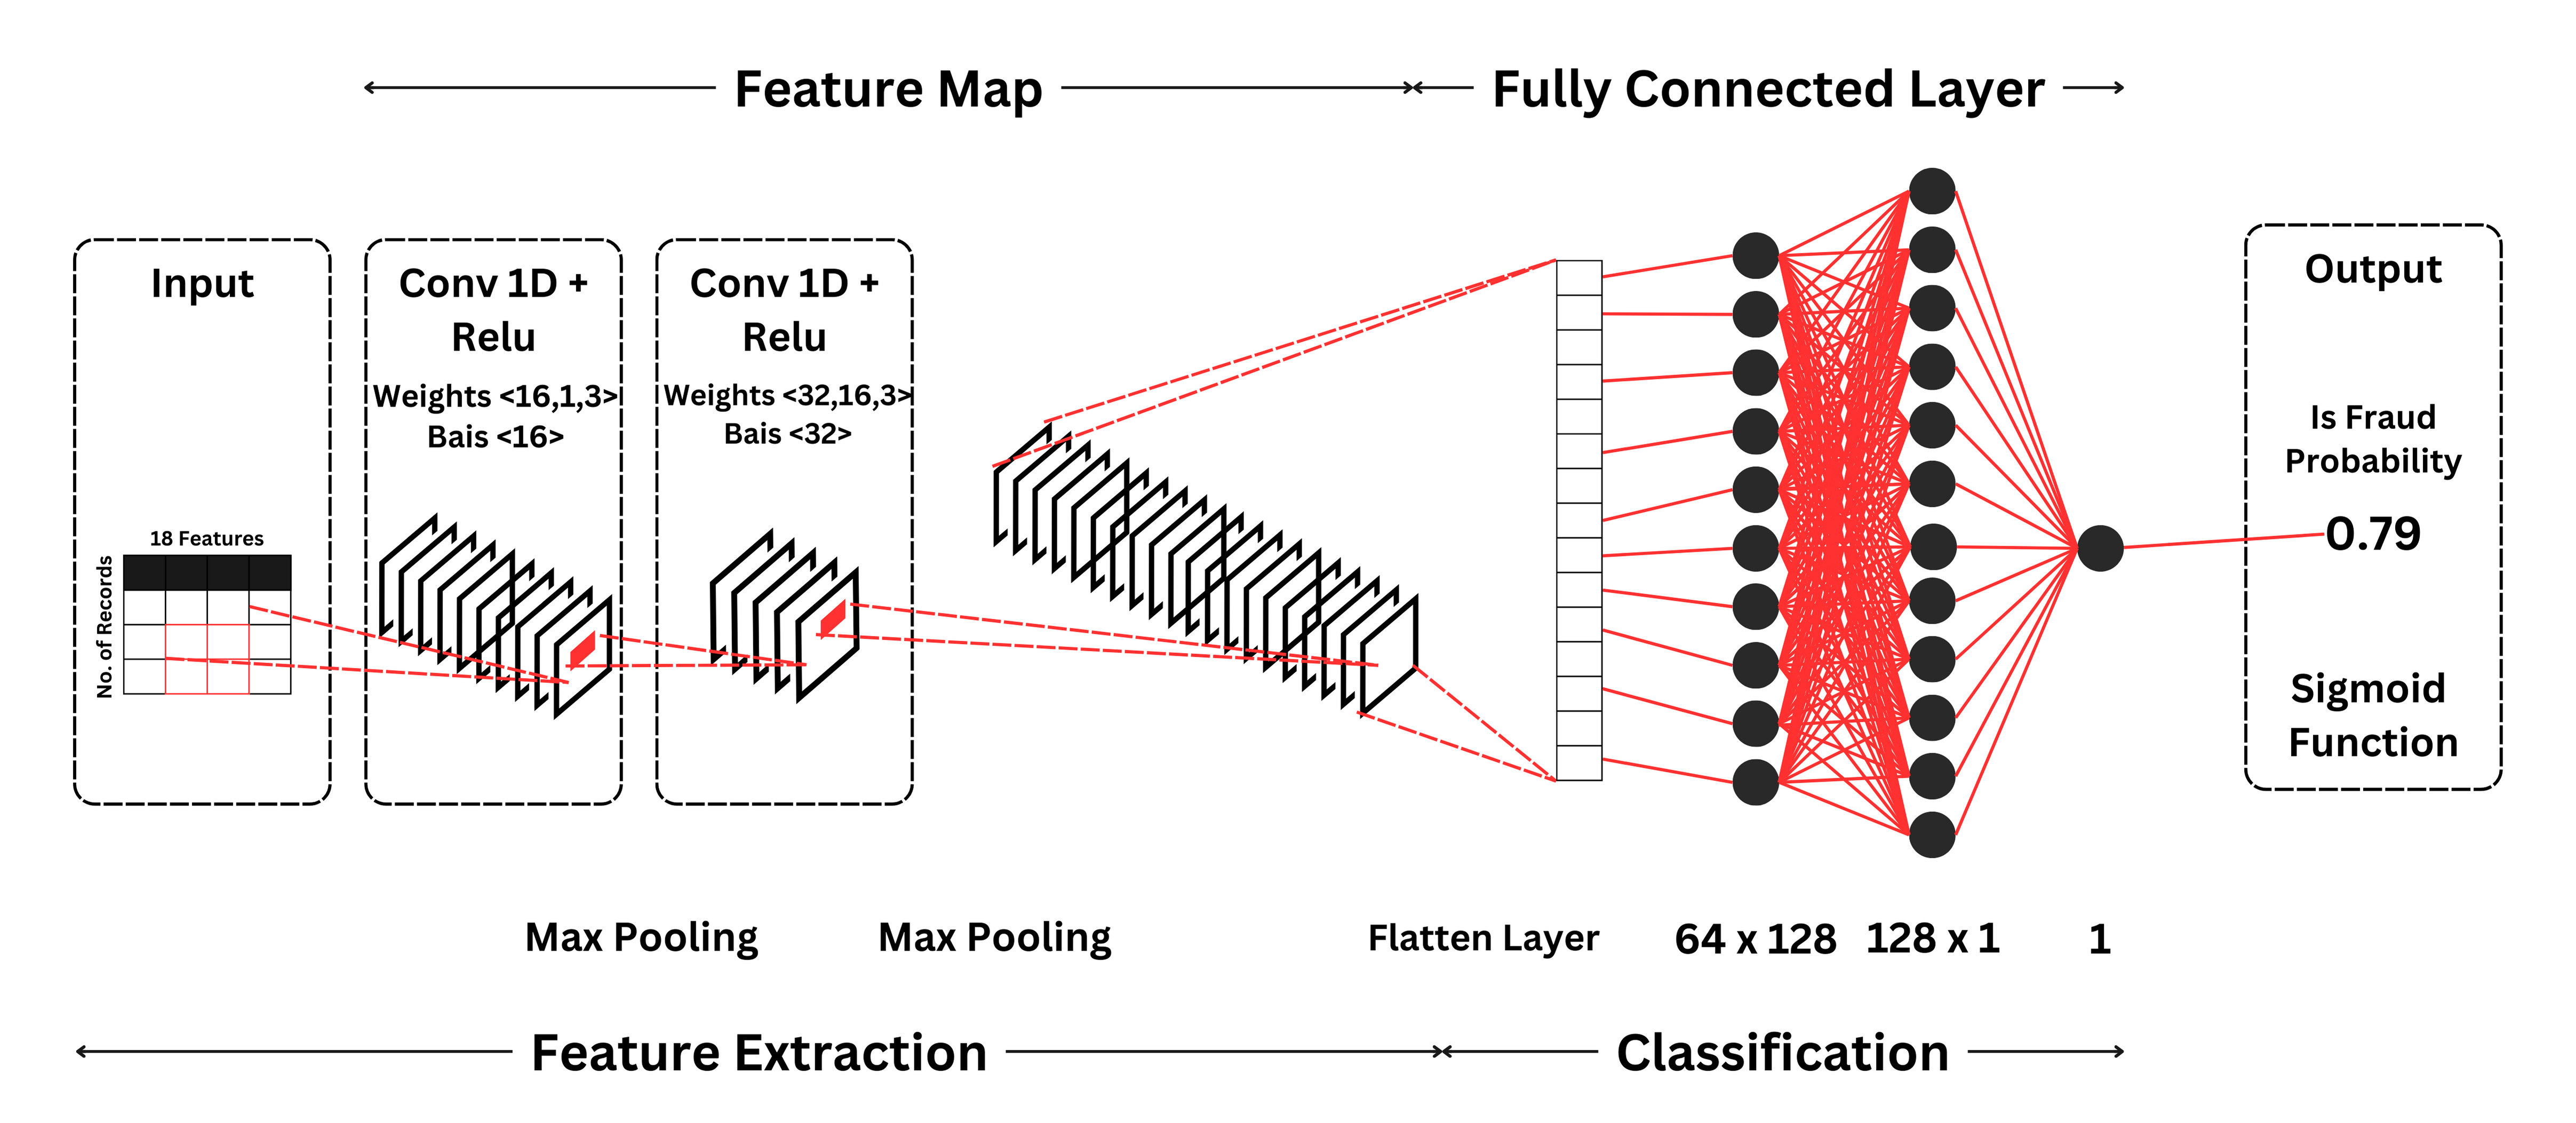
\includegraphics[width=1.0\textwidth]{CNN Model Architecture.png}
\caption{Architecture of the CNN model}\label{fig1}
\end{figure}

\item LSTM: Long Short-Term Memory networks, a type of recurrent neural network (RNN) that is equipped with memory cells capable of capturing long-range dependencies in sequential data, commonly applied in natural language processing and time series forecasting tasks. LSTMs excel at processing sequential data, making them promising for detecting fraudulent patterns over transaction histories and timestamps. The LSTM's memory cells can track evolving fraud signals. The key equations are as follows:

\begin{equation}
Input \hspace{0.1cm} Gate: i_t=\sigma\left(W_i\left[x_t,h_{t-1}\right]+b_i\right)
\end{equation}

\begin{equation}
Forget \hspace{0.1cm} Gate: f_t=\sigma\left(W_f\left[x_t,h_{t-1}\right]+b_f\right)
\end{equation}

\begin{equation}
Output \hspace{0.1cm} Gate: o_t = o_t=\sigma\left(W_o\left[x_t,h_{t-1}\right]+b_o\right) 
\end{equation}

\begin{equation}
Cell \hspace{0.1cm} State: C_t=f_t\odot C_{t-1}+i_t\odot\tanh{\left(W_C\left[x_t,h_{t-1}\right]+b_C\right)}
\end{equation}

\begin{equation}
Hidden \hspace{0.1cm} State: h_t=o_t\odot\tanh{\left(C_t\right)}
\end{equation}

The input, forget, and output gates control the flow of information into and out of the cell state  $C_t$, which is updated based on the previous cell state $C_{t-1}$ and the current input $x_t$. The hidden state $h_t$ is then computed as a filtered version of the updated cell state, modulated by the output gate. This allows the LSTM to selectively remember and forget information from the input sequence.

\clearpage

\begin{figure}[h]
\centering
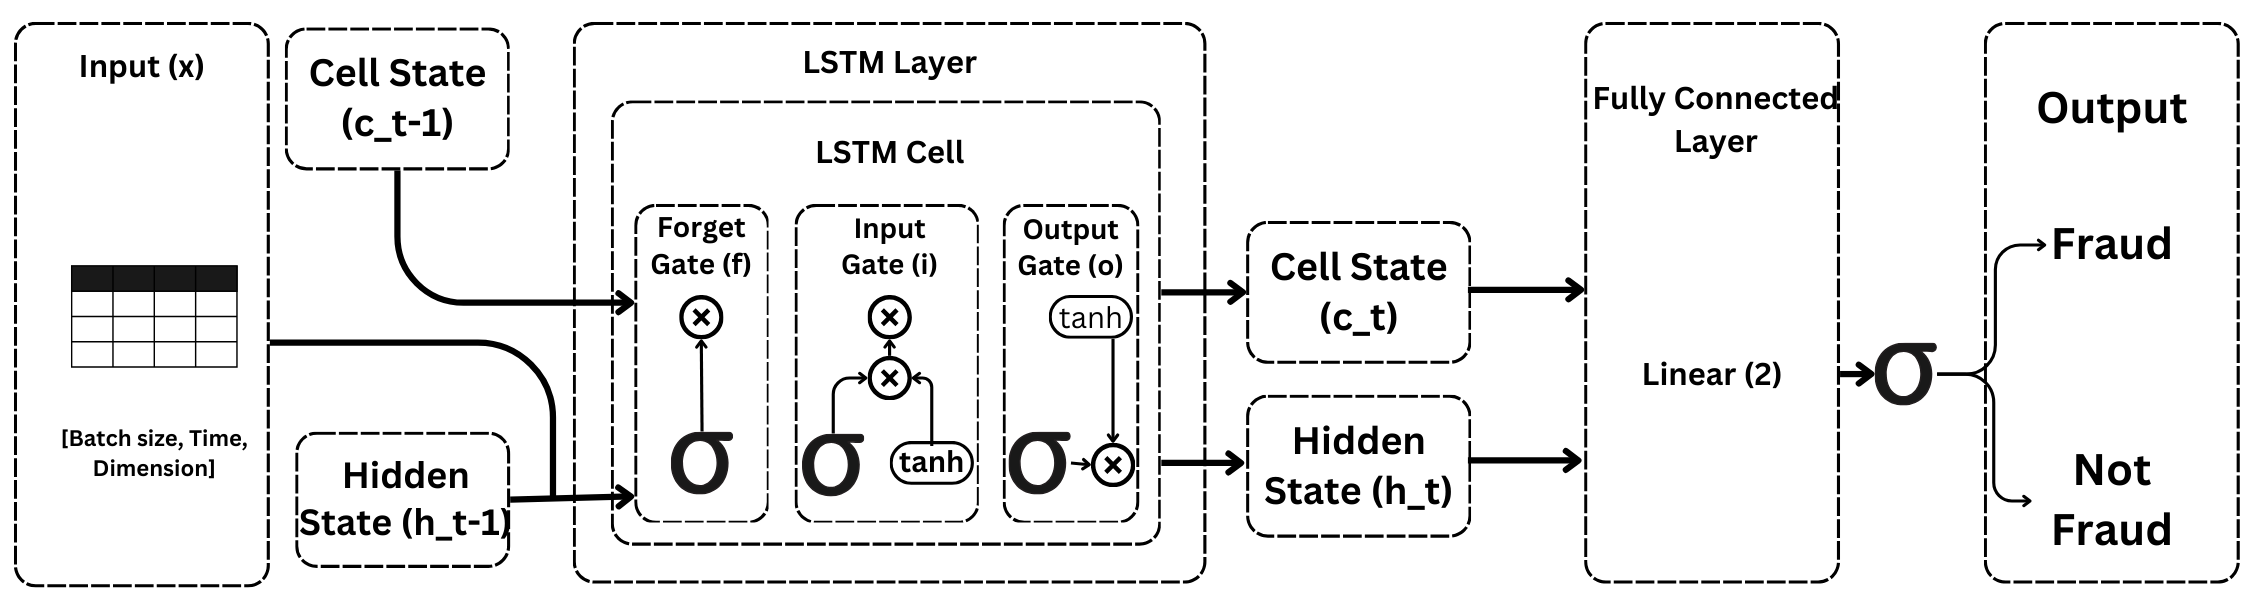
\includegraphics[width=1.0\textwidth]{LSTM Model Architecture.png}
\caption{Architecture of the LSTM model}\label{fig1}
\end{figure}




\item CNN-LSTM: A CNN-LSTM hybrid leverages the strengths of both architectures. The CNN first extracts salient features from the raw transaction fields. The LSTM then processes the resulting feature sequences. The CNN compresses information while the LSTM analyzes temporal relationships. This can identify suspicious merchant sequences or spending patterns over time.

For fraud detection, the CNN would learn to recognize concerning patterns within individual transactions, as in the pure CNN case. However, rather than making an immediate prediction, it would pass these learned features to the LSTM. The LSTM would then analyze the temporal evolution of these patterns across the user's transaction history. This allows detecting more subtle, long-term fraud schemes.

\end{enumerate}

\subsection{Graph Neural Networks}\label{subsec3}

\subsubsection{Graph Construction}\label{subsubsec3}

In response to the limitations observed in both homogenous graphs, where transactions solely serve as nodes, and in graphs where transactions are edges between source (card ID) and destination (merchant ID) nodes—primarily concerning static attributes and the loss of features—we've implemented a solution: the construction of a heterogeneous graph with learnable parameters. In this graph representation, the focal point is the transaction node, while the source and destination nodes correspond to the card ID and merchant ID, respectively. This approach imbues the transaction node with transaction-specific features, also known as node features, thereby enriching the graph's representational power. The source and destination nodes, i.e., card and merchant IDs, intentionally lack inherent features and are treated as learnable parameters. This strategic design allows for greater flexibility and adaptability within the model. Our classification task centres on predicting the transaction node, thereby making it a node classification problem. This framework not only addresses the shortcomings of existing graph representations but also paves the way for more effective and versatile analysis within complex transactional networks.

\textbf{Definition. Heterogeneous Graph:} Let us denote a heterogeneous directed graph as $G = (V, E, R, \phi)$, where:
\begin{itemize}
    \item $V$ is the set of nodes, which in our case is card IDs, merchant IDs, and transactions,
    \item $E$ is the set of edges, representing relationships between the nodes,
    \item $R$ is the set of relation types, indicating the type of relationship between nodes,
    \item $\phi$ is a node-type mapping function that assigns a type to each node in $V$, i.e., $\phi(v) = \tau$, where $\tau$ is the node type.
\end{itemize}

The edges in $E$ are defined as: $e(u, r, v) \in E$, where $u, v \in V$ are nodes, and $r \in R$ is the relation type or edge label.

In the context of our fraud detection graph, we can have different node types, such as: $\phi(u) = \text{card}$, for card ID nodes `$u$'; $\phi(v) = \text{merchant}$, for merchant ID nodes `$v$'; $\phi(t) = \text{transaction}$, for transaction nodes `$t$'. 

We also have different relation types, such as: $r = \text{source}$, for edges connecting a card ID to a transaction; and $r = \text{destination}$, for edges connecting a transaction to a merchant ID.

We use $X$ of size $t_n \times f$ to represent the feature matrix of the transaction nodes where $t_n$ is the number of transaction nodes and $f$ is the number of features.

\begin{figure}[h]
\centering
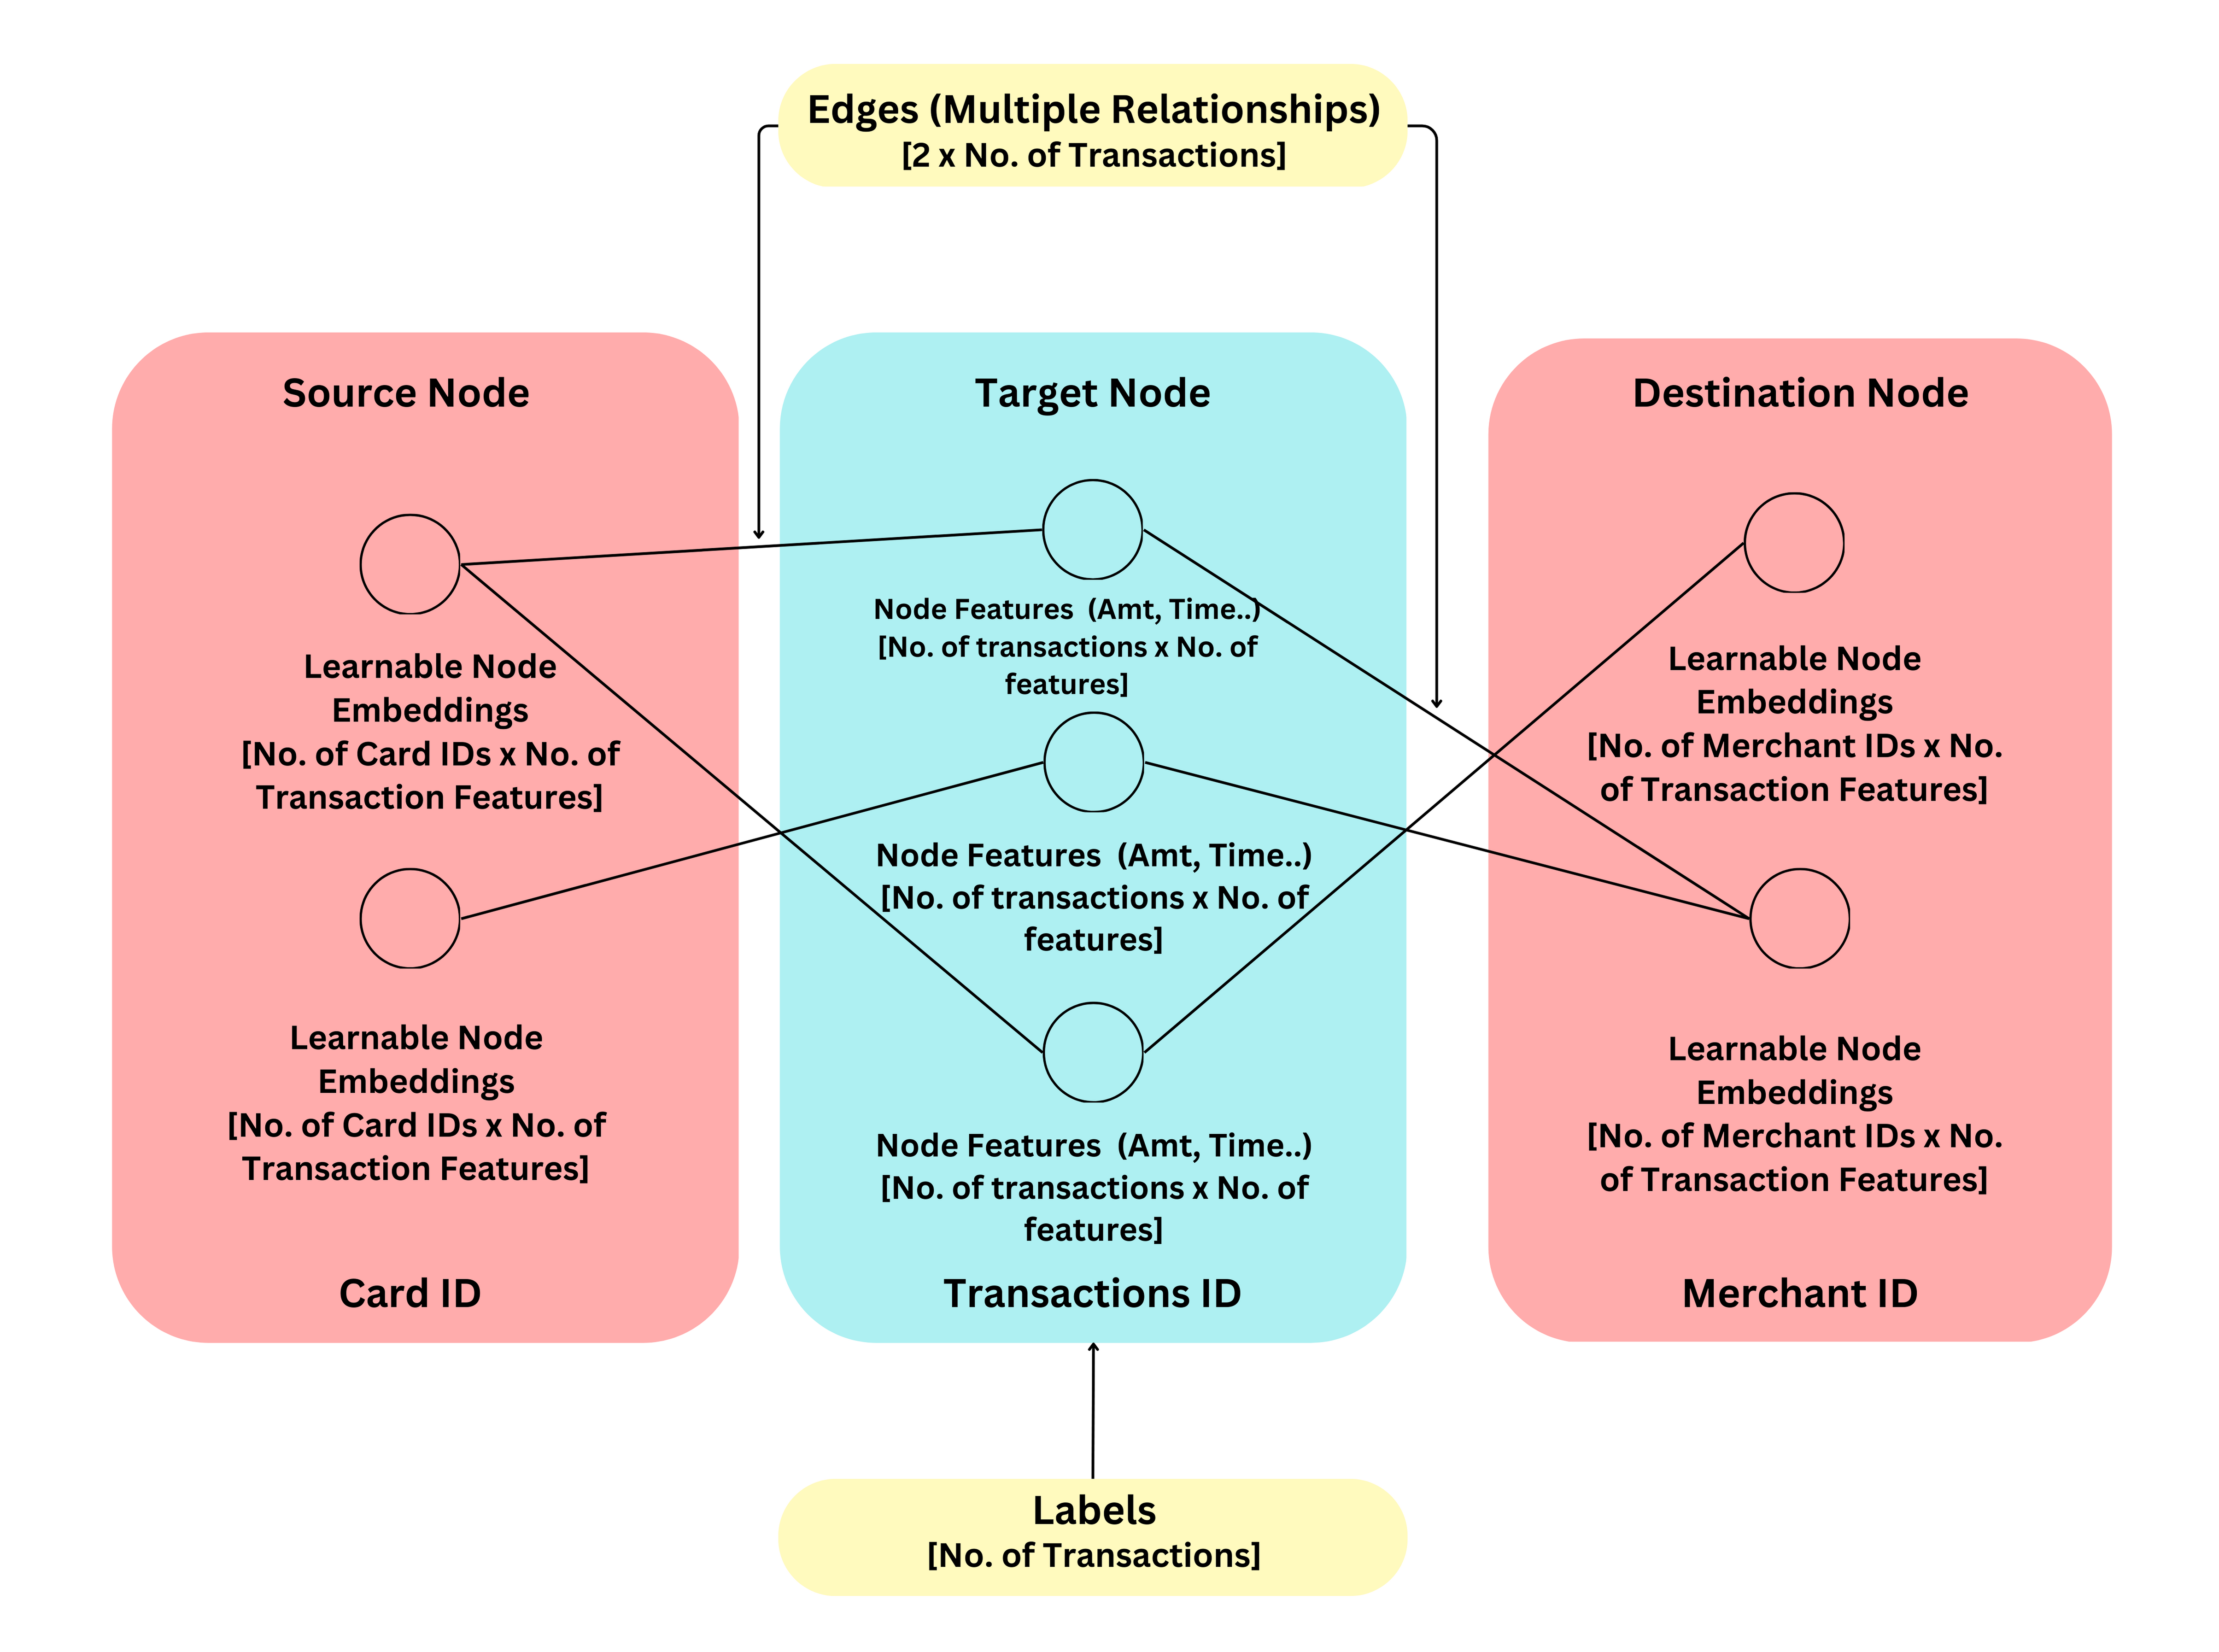
\includegraphics[width=1.0\textwidth]{graph_architecture.png}
\caption{Structure of the constructed Heterogenous graph}\label{fig1}
\end{figure}

\subsubsection{Message passing in GNN’s}\label{subsubsec3}

GNNs are known for their ability to learn structural information. Usually, nodes with similar features or properties are connected to each other. Information is propagated between the nodes of the graph structure. This process is called message passing and it aims to update the node representation incorporating the information from neighbouring nodes \cite{anand2022}. To do so, the GNN looks at the neighbourhoods of nodes.

The Neighbourhood $\mathcal{N}_i$ of a node $i$ is defined as the set of nodes $j$ connected to $i$ by an edge. The equation is as follows:

\begin{equation}
\mathcal{N}_{i =} \left\{ j : e_{ij} \in E \right\}
\end{equation}

Once we obtain the transformed messages, we aggregate them. Aggregations can be done using Sum, Mean, Min or Max. The equation for aggregation using Sum is as follows:

\begin{equation}
Sum=\ \sum_{j\in N_i} W_jx_j
\end{equation}

After aggregating messages from the neighbouring nodes, the GNN layer needs to update the feature representation of the source node i itself. The updated representation should not only encode the node's own features but also incorporate the information from its neighbours captured through the aggregated messages. This is achieved by combining the source node i 's original feature vector with the aggregated neighbourhood messages.
The equation for update using addition is as follows:

\begin{equation}
h_i=\ \sigma(K(H(x_i)\ +\bar{m}_i )))
\end{equation}


Now let us put the message passing, aggregation and updation formulae together for a single GNN layer on a single node $i$ to get our final equation:

\begin{equation}
h_i=\ \sigma(W_1.h_i+\sum_{j\in N_i} W_{2\ .}h_j)
\end{equation}


\subsubsection{Heterogenous RGCN}\label{subsubsec3}

R-GCNs are an extension of standard Graph Convolutional Networks (GCNs) designed to handle graphs with different types of relationships or edges between nodes (known as relational or heterogeneous graphs) \cite{schlichtkrull2018} \cite{fan2023}. The core idea is to perform message passing and neighbourhood aggregation while taking into account the different relation types present in the graph. The message-passing equation is as follows:

\begin{equation}
h_i^{\left(l+1\right)}=\ \sigma\left(\sum_{r\in R}\sum_{j\in N_r\left(i\right)}{W_r^{\left(l\right)}h_j^{\left(l\right)}}\right)
\end{equation}

Here: $h_i^{(l+1)}$  is the feature representation of node $i$ at the $l_{th}+1$ layer of the GCN, R is the set of all relation types (edge types) in the heterogeneous graph, $N_r(i)$ is the set of neighbor nodes of node $i$ under the relation $r$. $W_r^{(l)}$ is a learnable weight matrix specific to the relation type $r$ at layer $l$. $\sigma$  is a non-linear activation function like ReLU.

The message passing happens in two key steps: 

\begin{enumerate} [label=(\roman*),itemsep=10pt]


\item Per-edge-type Message Computation and Aggregation: For each relation type $r \in R$, the model computes messages by applying the relation-specific weight $W_r^{(l)}$ to the representations $h_i^{(l+1)}$ of all neighbouring nodes $j\in N_r(i)$. These weighted messages are then aggregated (summed up) to capture the neighbourhood information for node i under the relation r.

\item Type-wise Reduction: After computing and aggregating messages for each relation type r independently, the results are combined (reduced) by taking a sum across all relation types.

\end{enumerate}

So, the overall computation involves applying relation-specific transformations to neighbour representations, aggregating these transformed messages per relation type and lastly combining the per-relation aggregates into a single representation for the target node.

This allows the R-GCN to effectively propagate and integrate information along different types of edges/relations in the heterogeneous graph during the message passing process. The relation-specific weights $W_r^{(l)}$ enable the model to learn distinct transformation parameters for each edge type, capturing their unique neighborhood interaction patterns.

By performing this type-aware message passing, R-GCN can learn rich node representations that utilise both node features and multi-relational graph structure information present in heterogeneous graphs.

We apply the R-GCN model to the constructed heterogeneous graph to learn representations for classifying the transaction nodes of interest. The R-GCN performs relational message passing by transforming node representations from neighbouring nodes under different relation types (e.g. card-to-transaction, merchant-to-transaction) using relation-specific weight matrices. These transformed neighbour messages are then aggregated through a normalized sum operation into updated node representations. For the target transaction node, its embedding is computed by combining its initial node features with the aggregated multi-relational neighbourhood messages passing through a non-linear activation. This relational message passing, and aggregation process is parallelized across all nodes in the graph.

\clearpage

\begin{figure}[h]
\centering
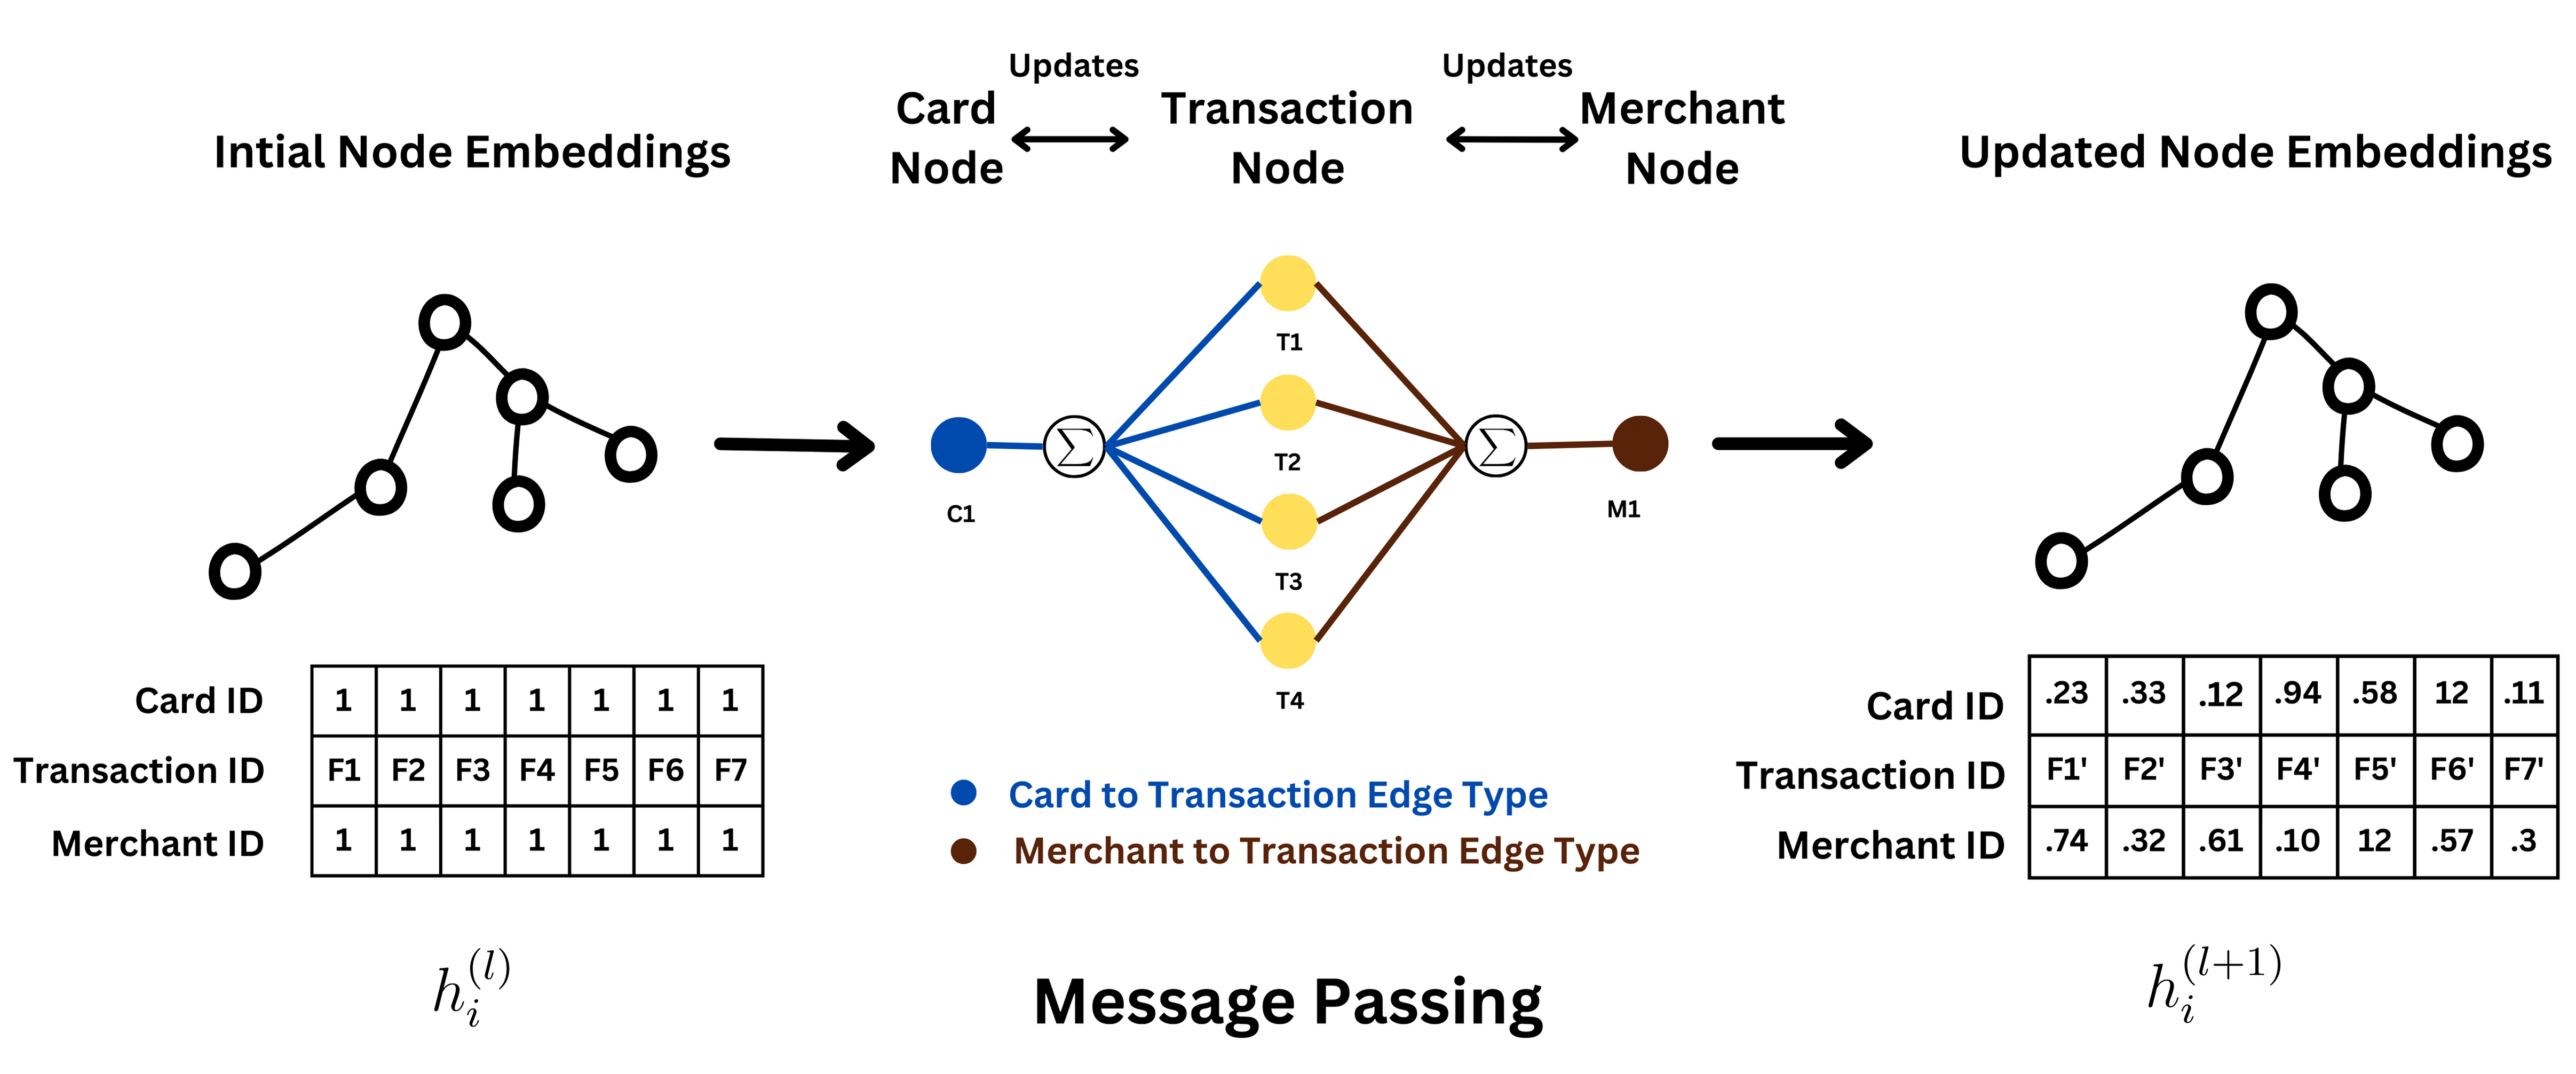
\includegraphics[width=1.0\textwidth]{RGCN_message_passing.png}
\caption{The diagram above depicts the message passing mechanism in a Relational Graph Convolutional Network (RGCN) }\label{fig3}
\end{figure}


The figure provides an illustration of the initial node embeddings for Card ID, Transaction ID, and Merchant ID nodes which are updated by propagating and aggregating information along the edges connecting these node types. This results in updated node embeddings that captures relational information from the graph structure



\section{Experiments and Results}\label{sec4}

\subsection{Dataset Description}\label{subsec4}

The dataset we have used to conduct our study is a synthetic dataset provided by IBM \cite{ibm2021}. The dataset consists of 24 million unique transactions, involving 6,139 unique cards and 100,343 unique merchants. Among these transactions, 29,757 are labelled as fraudulent, accounting for 0.1\% of the total transactions.

The highly imbalanced nature of the TabFormer dataset, with a significantly lower proportion of fraudulent transactions compared to legitimate ones, is a common characteristic of real-world fraud detection scenarios. This imbalance poses challenges for anomaly detection models, as they need to effectively identify the rare fraudulent instances while minimizing false positives.
The TabFormer dataset provides a realistic representation of financial transaction data, enabling researchers and practitioners to develop and evaluate anomaly detection models in a controlled environment. The dataset's large scale and imbalanced distribution make it suitable for benchmarking the performance of various anomaly detection techniques, including traditional machine learning models, deep learning architectures, and graph neural networks.

\subsection{Dataset Preprocessing}\label{subsec4}

The Tabformer dataset undergoes several preprocessing steps in order to ensure data quality and prepare it for the comparative study on our models. The preprocessing pipeline is implemented using a custom function which takes the dataset as input along with various parameters to control the preprocessing steps.

Firstly, the function automatically detects columns with only two unique values and encodes them as binary (0 and 1). This step helps in representing binary features effectively. Next, the columns are converted to numeric data type, when possible, to ensure consistent data representation across the dataset. To handle categorical variables, the non-numeric columns are one-hot encoded, converting them into binary vectors. This encoding technique allows the models to process categorical data effectively. Missing values in the dataset are handled by replacing them with the mode (most frequent value) of each column, ensuring that no data points are lost due to missing information.

To reduce the dataset's size while maintaining the class distribution, stratified sampling is applied based on the 'Is Fraud?' column. This step helps in creating a representative sample of both fraudulent and non-fraudulent transactions. The 'Time' column, which contains datetime information, is treated separately, and appropriate datetime features are extracted from it. Data cleaning is performed on specific columns to ensure data consistency. The 'Amount' column undergoes cleaning to remove any special characters or inconsistencies. Additionally, columns that may not be relevant for anomaly detection, such as 'Card', 'User', and 'Merchant Name', are removed from the dataset. Certain columns, including 'Use Chip', 'Merchant City', 'Merchant State', 'Zip', 'MCC', and 'Errors?', are considered as categorical variables and are encoded accordingly. The 'Is Fraud?' column is designated as the target variable for the anomaly detection task.

It is worth noting that normalization and class balancing techniques are not applied in this preprocessing pipeline. The preprocessing steps are carefully designed to clean, transform, and prepare the Tabformer dataset for the subsequent comparative study on anomaly detection models.

\subsection{Implementation}\label{subsec4}

For our study, we have sampled 60\% of the original data which is around 15 million due to memory constraints. We split the data into training, validation, and test data sets with the ratio 60:20:20. We have used Scikit-Learn (1.4.1), XGBoost (2.0.3), Pytorch (2.2.0) and DGL (0.9.1) for our study. For our deep learning models, we have used a learning rate of 0.0001 and Adam optimizer with number of epochs set to 300 and a batch size of 512.

For GNN’s, we have used a learning rate of 0.01 with hidden dimensions 16 and a weight decay of 5e-4. Adam optimizer is used to optimize the parameters and the number of epochs is set to 1000. The loss function used in both cases is CrossEntropyLoss.

\subsection{Results}\label{subsec4}

Comparing the various methods used and choosing the best model is an important part of developing an effective and reliable system for credit card fraud detection. Since credit card fraud datasets are highly imbalanced, it is important to choose the appropriate evaluation metrics. In this study, we have selected four metrics F1-Score, Precision, Recall and AUCPR as they focus on capturing the true positives predicted. Our \textbf{main metric is the F1 score} which is the harmonic mean of precision and recall. Our \textbf{2nd important metric is Recall} as it measures the ability of the model to correctly identify fraudulent transactions among all actual fraudulent transactions. 

To prove that our approach with Graph Neural Networks can perform better than classical and deep learning models we run a comparison study on using all the models and calculate the evaluation metrics.

The results are as follows:

\begin{table}[h]
\caption{Results of different models on the IBM Tabformer Dataset}\label{tab1}%
\begin{tabular}{@{}lllll@{}}
\toprule
Methods & Precision  & Recall & F1-Score & AUCPR\\
\midrule
Logistic Regression    & 0.63   & 0.13  & 0.22 & 0.18  \\
Random Forest    & 0.97   & 0.51  & 0.67 & 0.76  \\
LightGBM  & 0.71   & 0.50  & 0.58 & 0.45  \\
CatBoost    & \textbf{0.96}   & 0.63  & 0.76 & \textbf{0.80}  \\
XGBoost    & 0.95   & 0.63  & 0.76 & \textbf{0.80}   \\
CNN    & 0.85   & 0.45  & 0.59 & 0.60   \\
LSTM    & 0.91   & 0.45  & 0.61 & 0.63   \\
CNN-LSTM    & 0.82   & 0.56  & 0.67 & 0.68   \\
GNN    & 0.94   & \textbf{0.66}  & \textbf{0.78} & 0.78   \\
\botrule
\end{tabular}
\end{table}

Looking at the performances of our fraud detection model, the classical models Logistic Regression performs the worst among all. This might be because LR is biased more towards the majority class and is unable to handle data imbalance. The performance of XGBoost and CatBoost are almost similar to each other with an F1-Score of 0.76, and they perform the best among the machine learning models. This is in line with our research that XGBoost can handle imbalanced data well.

Coming to the Deep Learning models, CNN and LSTM have performed well compared to LR and LightGBM. Our ensemble method using CNN and LSTM has performed better than CNN and LSTM alone and is also in line with the F1 Score (0.67) of Random Forest model.

Lastly, Graph Neural Networks have performed better than the other models with an F1 Score of 0.78 and a recall rate of 0.66.

In summary GNN has achieved better results compared to classical and deep learning methods when it comes to solving the problem of credit card fraud detection.

\clearpage


\begin{figure*}
    \centering
    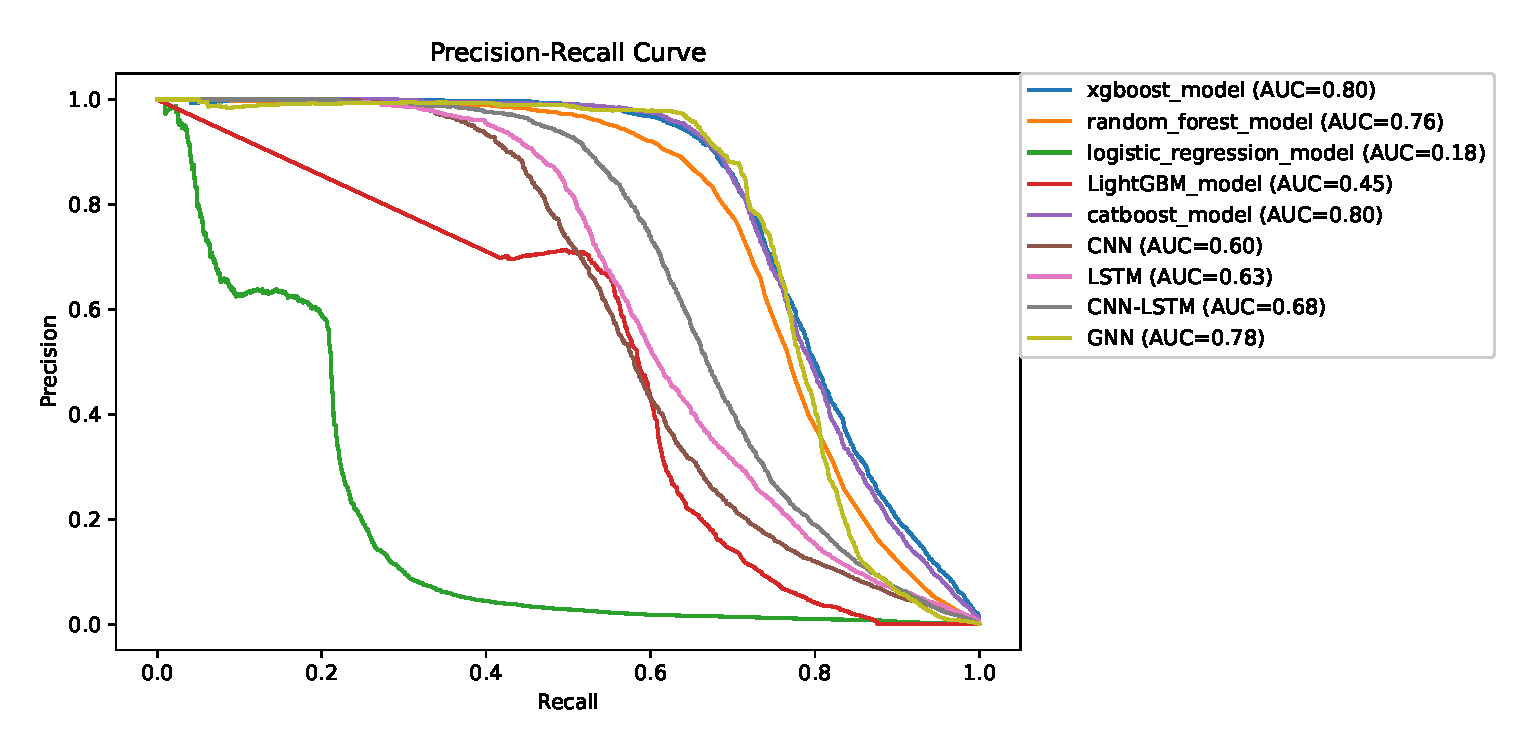
\includegraphics[width=1.0\textwidth]{AUCPR_Curve.eps}
    \caption{AUCPR curves for Classical, Deep Learning and GNN models}
\end{figure*}


\section{Conclusions and Future Work}\label{sec5}

In conclusion, this paper presents an approach to address the limitations of existing graph representations in transactional networks by introducing a heterogeneous graph framework. By structuring the graph with transaction nodes as the focal point and incorporating learnable parameters for card and merchant ID nodes, our model enhances the representation of transactional data and improves classification performance. Through experimentation, we demonstrate the effectiveness of Graph Neural Networks when compared to other methods, showcasing its potential for various applications in fraud detection, recommendation systems, and beyond.

For future work, incorporating sampling strategies and edge weights into our heterogeneous graph framework represents a promising direction offering opportunities to enhance scalability, efficiency, and predictive performance in transactional network analysis and related domains. Further, integrating attention mechanisms into our heterogenous graph to allow nodes to focus on relevant neighbours during message passing can enhance the ability to capture complex relationships.

\section{Statements and Declarations}\label{sec6}

\textbf{Conflicts of interest.} I hereby certify that to the best of my knowledge,the authors have no relevant financial or non-financial interests to disclose. The authors have no conflicts of interest to declare that are relevant to the content of this article. All authors certify that they have no affiliations with or involvement in any organization or entity with any financial interest or non-financial interest in the subject matter or materials discussed in this manuscript. The authors have no financial or proprietary interests in any material discussed in this article. 

\textbf{Data Availability.} The data that supports the findings of this study are available in the Github Repository at \url{https://github.com/IBM/TabFormer/tree/main/data/credit_card}

%%===========================================================================================%%
%% If you are submitting to one of the Nature Portfolio journals, using the eJP submission   %%
%% system, please include the references within the manuscript file itself. You may do this  %%
%% by copying the reference list from your .bbl file, paste it into the main manuscript .tex %%
%% file, and delete the associated \verb+\bibliography+ commands.                            %%
%%===========================================================================================%%

\bibliography{sn-bibliography}% common bib file
%% if required, the content of .bbl file can be included here once bbl is generated
%%\input sn-article.bbl


\end{document}
